\chapter{Phân tích Biến đôi và Phân tích Đường cong Lợi suất}
\label{ch:M1L4}

\section*{Lesson Notes}

\textbf{Dự án} \\
\textbf{Thời gian đọc:} 60 phút \\
\textbf{Kiến thức nền tảng:} Trái phiếu Kho bạc Hoa Kỳ (U.S. Treasury Bonds), Đường cong lợi suất (Yield Curve), Đại số tuyến tính (Linear Algebra), Python cơ bản \\
\textbf{Từ khóa:} Đường cong giá-lợi suất trái phiếu (Bond price-yield curve), Lãi suất phi rủi ro (Risk free interest rate), Nelson Siegel, Spline bậc ba (Cubic Spline)

Trong bài học trước, chúng ta đã giới thiệu về đường cong giá - lợi suất Trái phiếu Kho bạc Hoa Kỳ và thảo luận về hình dáng của đường cong này. Chúng ta cũng đã tìm hiểu các phương pháp để khớp đường cong Kho bạc Hoa Kỳ bằng cách sử dụng các kỹ thuật khớp đa thức. Trong bài học này, chúng ta sẽ tiếp tục học các phương pháp phân tích mới để hiểu rõ hơn về lợi suất Trái phiếu Kho bạc Hoa Kỳ. Đầu tiên, chúng ta sẽ khám phá các mối quan hệ biến đôi (bivariate relationships) của các mức lợi suất khác nhau, bao gồm tương quan (correlation) và hiệp phương sai (covariance). Sau đó, chúng ta sẽ học một kỹ thuật mới để trích xuất các đặc điểm chính của đường cong lợi suất Kho bạc Hoa Kỳ nhằm phân tích hành vi của đường cong này.

\section[Phân tích Biến đôi]{Phân tích Biến đôi (Bivariate Analysis)}

Phân tích biến đôi là một tập hợp các phương pháp nhằm phân tích mối quan hệ giữa hai biến số. Trong tài chính, chúng ta đặc biệt quan tâm đến việc hiểu cách hai biến số tương tác với nhau. Trong bài học này, chúng ta sẽ xem xét lợi suất của các Trái phiếu Kho bạc Hoa Kỳ khác nhau và cách chúng dịch chuyển trong mối tương quan lẫn nhau. Công cụ phân tích biến đôi đầu tiên chúng ta sẽ học là hiệp phương sai (covariance).

\subsection[Hiệp phương sai]{Hiệp phương sai (Covariance)}

Hiệp phương sai là một thước đo để đánh giá mức độ dịch chuyển cùng nhau của hai biến số. Cụ thể, hiệp phương sai tính toán độ lớn của biến động mà hai biến số thể hiện. Dưới đây là công thức tính hiệp phương sai:

$$Cov(X,Y)=E[(X-E[X])(Y-E[Y])]$$

Dưới đây là một số tính chất của hiệp phương sai:
1. Nếu hiệp phương sai mang dấu dương, điều đó có nghĩa là hai biến số dịch chuyển cùng chiều.
2. Nếu hiệp phương sai mang dấu âm, hai biến số dịch chuyển ngược chiều nhau.
3. Nếu hiệp phương sai bằng 0, hai biến số không có tương quan tuyến tính (uncorrelated).

Giá trị tuyệt đối của hiệp phương sai giữa hai biến số càng cao, mối quan hệ (dương hoặc âm) giữa hai biến số càng mạnh. Hãy cùng trích xuất một số dữ liệu lợi suất Trái phiếu Kho bạc Hoa Kỳ để minh họa cho hiệp phương sai giữa hai mức lợi suất khác nhau.

Ma trận hiệp phương sai là một thước đo phân tích biến đôi cho hai biến số. Tuy nhiên, khi chúng ta có một số lượng biến lớn hơn và muốn biết mối quan hệ theo cặp của các biến này, chúng ta sẽ cần đến một ma trận hiệp phương sai (covariance matrix). Ma trận hiệp phương sai là một ma trận vuông thể hiện các hiệp phương sai theo cặp giữa nhiều biến số trong một tập dữ liệu. Bây giờ, hãy trích xuất dữ liệu lợi suất Trái phiếu Kho bạc Hoa Kỳ và điều tra ma trận hiệp phương sai của chúng.

\begin{lstlisting}[language=Python]
In [1]: import pandas as pd
        from fredapi import Fred
        import matplotlib.pyplot as plt
        import seaborn as sns
        sns.set()
\end{lstlisting}

\begin{lstlisting}[language=Python]
In [2]: # Initialize the FRED API with your key
        fred = Fred(api_key='5079f41d061a4037d81f3da69e018803') # Replace my APIKEY
        # List of Treasury yield series IDs
        series_ids = ['DGS1MO', 'DGS3MO', 'DGS6MO', 'DGS1', 'DGS2', 'DGS3', 'DGS5',
                      'DGS7', 'DGS10', 'DGS20', 'DGS30']
                      
        # Function to get data for a single series
        def get_yield_data(series_id):
            data = fred.get_series(series_id, observation_start="1975-01-01", observ
            return data
            
        # Get data for all series
        yields_dict = {series_id: get_yield_data(series_id) for series_id in series_
        
        # Combine into a single DataFrame
        yields = pd.DataFrame(yields_dict)
        
        # Rename columns for clarity
        yields.columns = ['1 Month', '3 Month', '6 Month', '1 Year', '2 Year', '3 Ye
                          '7 Year', '10 Year', '20 Year', '30 Year']
\end{lstlisting}

\begin{lstlisting}[language=Python]
In [3]: # Make datetime as the index
        yields.index = pd.to_datetime(yields.index)
\end{lstlisting}

\begin{lstlisting}[language=Python]
In [4]: # Drop NaN in the dataset
        yields = yields.dropna()
\end{lstlisting}

\begin{lstlisting}[language=Python]
In [5]: # Calculate covariance matrix for US Treasury yields in the dataset
        covariance_matrix = yields.cov()
        print("Covariance Matrix:")
        print(covariance_matrix)
\end{lstlisting}

\begin{lstlisting}[language=Python]
Covariance Matrix:
         1 Month   3 Month   6 Month    1 Year    2 Year    3 Year    5 Year \
1 Month  2.909927  2.946278  2.948709  2.812408  2.499031  2.251515  1.850674
3 Month  2.946278  3.004493  3.018967  2.887166  2.571375  2.317856  1.901841
6 Month  2.948709  3.018967  3.051413  2.931246  2.624882  2.372696  1.951042
1 Year   2.812408  2.887166  2.931246  2.836161  2.569272  2.340278  1.944752
2 Year   2.499031  2.571375  2.624882  2.569272  2.388302  2.216908  1.897526
3 Year   2.251515  2.317856  2.372696  2.340278  2.216908  2.092766  1.842915
5 Year   1.850674  1.901841  1.951042  1.944752  1.897526  1.842915  1.714387
7 Year   1.565717  1.605385  1.647697  1.654011  1.648671  1.634697  1.582433
10 Year  1.315260  1.344596  1.381242  1.395294  1.418752  1.435157  1.447139
20 Year  1.078020  1.098030  1.128773  1.154327  1.214425  1.267258  1.350980
30 Year  0.862766  0.872645  0.893530  0.919017  0.988536  1.052167  1.161403

         7 Year    10 Year   20 Year   30 Year
1 Month  1.565717  1.315260  1.078020  0.862766
3 Month  1.605385  1.344596  1.098030  0.872645
6 Month  1.647697  1.381242  1.128773  0.893530
1 Year   1.654011  1.395294  1.154327  0.919017
2 Year   1.648671  1.418752  1.214425  0.988536
3 Year   1.634697  1.435157  1.267258  1.052167
5 Year   1.582433  1.447139  1.350980  1.161403
7 Year   1.504196  1.416231  1.371829  1.204537
10 Year  1.416231  1.378491  1.383803  1.238816
20 Year  1.371829  1.383803  1.455676  1.324389
30 Year  1.204537  1.238816  1.324389  1.229380
\end{lstlisting}

Từ ma trận hiệp phương sai cho lợi suất Trái phiếu Kho bạc Hoa Kỳ ở trên, chúng ta có thể thấy tất cả các lợi suất theo từng cặp đều có hiệp phương sai dương. Điều này có nghĩa là khi lợi suất của một kỳ hạn tăng, các mức lợi suất khác cũng sẽ tăng. Chúng ta có thể trực quan hóa ma trận hiệp phương sai bằng bản đồ nhiệt (heatmap) trong Python.

\begin{lstlisting}[language=Python]
In [6]: # Make a heatmap for covariance matrix
        plt.figure(figsize=(8, 6))
        sns.heatmap(covariance_matrix, annot=True, cmap="coolwarm", fmt=".1f")
        plt.title('Covariance Heat Map of Treasury Bond Yields')
        plt.show()
\end{lstlisting}

\begin{figure}[htbp]
    \centering
    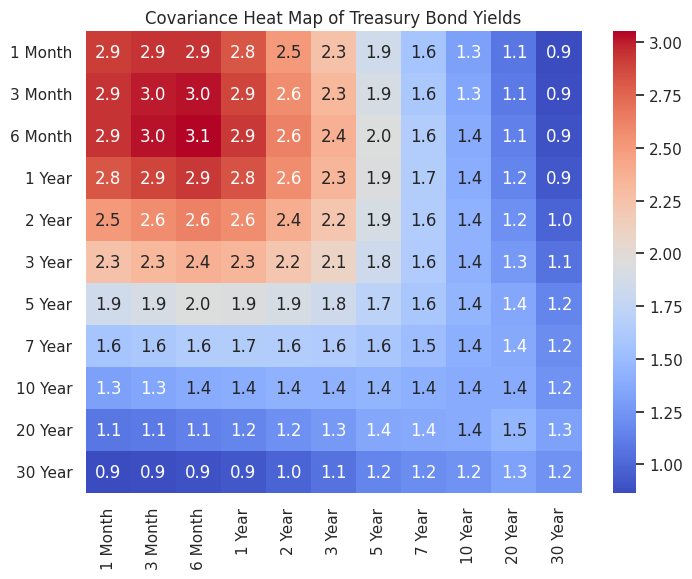
\includegraphics[width=1\textwidth]{gfx/m1l4_notes_covariance_heatmap.png}
    \caption{Bản đồ nhiệt Hiệp phương sai của Lợi suất Trái phiếu Kho bạc}
    \label{fig:m1l4_notes_covariance_heatmap}
\end{figure}

Từ bản đồ nhiệt ma trận hiệp phương sai ở trên, chúng ta có thể đọc các sự khác biệt về các giá trị hiệp phương sai một cách dễ dàng hơn. Tuy nhiên, một nhược điểm của hiệp phương sai là giá trị của nó thay đổi khi thang đo của hai biến số thay đổi. Chúng ta không thể đơn thuần so sánh các hiệp phương sai khác nhau cho các biến số theo cặp khác nhau để đánh giá xem chúng dịch chuyển cùng nhau chặt chẽ đến mức nào. Do vấn đề này, chúng ta sử dụng tương quan (correlation) thường xuyên hơn trong phân tích dữ liệu.

\subsection[Tương quan]{Tương quan (Correlation)}

Tương quan cũng là một thước đo để đánh giá sự dịch chuyển cùng chiều của hai biến số. Tuy nhiên, nó loại bỏ vấn đề về thang đo đã đề cập ở trên bằng cách chia hiệp phương sai cho căn bậc hai của tích phương sai của hai biến. Dưới đây là công thức toán học tính tương quan:

$$Corr(X,Y)=\frac{Cov(X,Y)}{\sqrt{Var(X)*Var(Y)}}$$

trong đó $Cov(X,Y)$ là hiệp phương sai của $X$ và $Y$, $Var(X)$ và $Var(Y)$ là phương sai của $X$ và $Y$.

Dưới đây là một số tính chất của tương quan:
1. Không giống như hiệp phương sai, giá trị của tương quan bị giới hạn trong khoảng từ -1 đến 1.
2. Nếu tương quan của hai biến lớn hơn 0, hai biến số có tương quan dương (positively correlated).
3. Nếu tương quan của hai biến nhỏ hơn 0, hai biến số có tương quan âm (negatively correlated).
4. Nếu hai biến có tương quan dương hoàn hảo, mức tương quan sẽ là 1.
5. Nếu hai biến có tương quan âm hoàn hảo, mức tương quan sẽ là -1.
6. Nếu mức tương quan bằng 0, hai biến không có tương quan tuyến tính.

Tương tự như với ma trận hiệp phương sai, nếu chúng ta có một số lượng biến lớn, chúng ta có thể sử dụng ma trận tương quan (correlation matrix) để trình bày các chỉ số tương quan cho các biến theo cặp. Hãy cùng tính toán ma trận tương quan cho dữ liệu lợi suất Trái phiếu Kho bạc Hoa Kỳ của chúng ta.

\begin{lstlisting}[language=Python]
In [7]: # Calculate correlation matrix for US Treasury yields in the dataset
        correlation_matrix = yields.corr()
        print("Correlation Matrix:")
        print(correlation_matrix)
\end{lstlisting}

\begin{lstlisting}[language=Python]
Correlation Matrix:
         1 Month   3 Month   6 Month   1 Year    2 Year    3 Year    5 Year \
1 Month  1.000000  0.996431  0.989556  0.978975  0.947951  0.912375  0.828580
3 Month  0.996431  1.000000  0.997062  0.989056  0.959920  0.924359  0.837981
6 Month  0.989556  0.997062  1.000000  0.996406  0.972332  0.938926  0.853025
1 Year   0.978975  0.989056  0.996406  1.000000  0.987188  0.960598  0.881951
2 Year   0.947951  0.959920  0.972332  0.987188  1.000000  0.991614  0.937754
3 Year   0.912375  0.924359  0.938926  0.960598  0.991614  1.000000  0.972950
5 Year   0.828580  0.837981  0.853025  0.881951  0.937754  0.972950  1.000000
7 Year   0.748376  0.755164  0.769085  0.800794  0.869836  0.921350  0.985414
10 Year  0.656702  0.660700  0.673469  0.705664  0.781916  0.844962  0.941356
20 Year  0.523785  0.525045  0.535579  0.568108  0.651319  0.726060  0.855190
30 Year  0.456151  0.454056  0.461334  0.492170  0.576905  0.655966  0.799992

         7 Year    10 Year   20 Year   30 Year
1 Month  0.748376  0.656702  0.523785  0.456151
3 Month  0.755164  0.660700  0.525045  0.454056
6 Month  0.769085  0.673469  0.535579  0.461334
1 Year   0.800794  0.705664  0.568108  0.492170
2 Year   0.869836  0.781916  0.651319  0.576905
3 Year   0.921350  0.844962  0.726060  0.655966
5 Year   0.985414  0.941356  0.855190  0.799992
7 Year   1.000000  0.983513  0.927076  0.885778
10 Year  0.983513  1.000000  0.976877  0.951616
20 Year  0.927076  0.976877  1.000000  0.990011
30 Year  0.885778  0.951616  0.990011  1.000000
\end{lstlisting}

Tiếp theo, hãy tạo một bản đồ nhiệt cho ma trận tương quan để dễ đọc kết quả hơn.

\begin{lstlisting}[language=Python]
In [8]: # Make a heatmap for correlation matrix
        plt.figure(figsize=(8,6))
        sns.heatmap(correlation_matrix, annot=True, cmap='coolwarm', fmt=".2f")
        plt.title('Correlation Heat Map of Treasury Bond Yields')
        plt.show()
\end{lstlisting}

\begin{figure}[htbp]
    \centering
    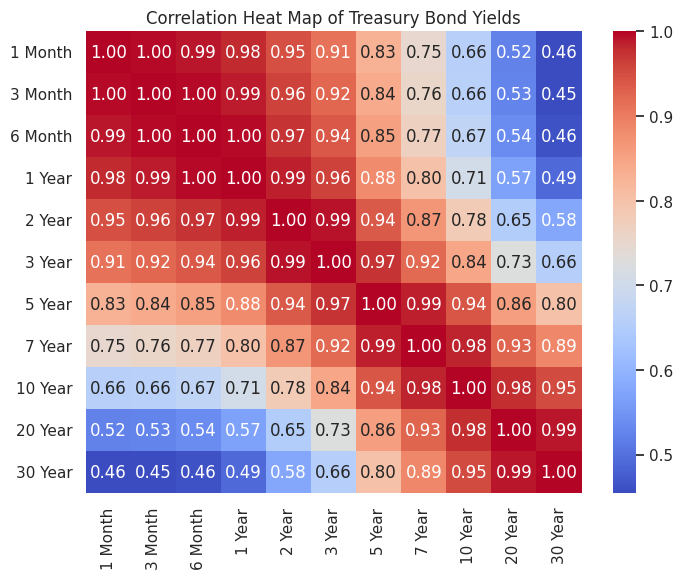
\includegraphics[width=1\textwidth]{gfx/m1l4_notes_correlation_heatmap.png}
    \caption{Bản đồ nhiệt Tương quan của Lợi suất Trái phiếu Kho bạc}
    \label{fig:m1l4_notes_correlation_heatmap}
\end{figure}

Từ bản đồ nhiệt ma trận tương quan cho lợi suất Trái phiếu Kho bạc Hoa Kỳ ở trên, chúng ta có thể so sánh tương quan giữa các cặp lợi suất khác nhau. Đầu tiên, chúng ta có thể thấy các giá trị tương quan trên các ô đường chéo đều là 1. Điều này dễ hiểu vì tất cả các mức lợi suất đều biến động hoàn toàn đồng điệu với chính nó. Thứ hai, một quan sát thú vị khác là hai lợi suất có kỳ hạn gần nhau thì có sự tương quan cao hơn. Khi khoảng cách về kỳ hạn của hai lợi suất ngày càng mở rộng, tương quan giữa hai mức lợi suất càng thấp.

Do tính chất dễ hiểu của nó, thước đo tương quan là một công cụ đo lường quan trọng và thường được sử dụng trong phân tích biến đôi. Hiểu được mối tương quan giữa lợi suất của các loại Trái phiếu Kho bạc khác nhau là điều rất quan trọng trong quản trị rủi ro, xây dựng danh mục đầu tư và thấu hiểu các động lực học của thị trường. Nó giúp định lượng cách các phần khác nhau của đường cong lợi suất dịch chuyển so với nhau, điều này đặc biệt cần thiết cho các chiến lược như giao dịch theo đường cong lợi suất và miễn nhiễm rủi ro (immunization) trong các danh mục đầu tư trái phiếu.

\section[Trích xuất Đặc trưng và Phân tích Thành phần Chính]{Trích xuất Đặc trưng và Phân tích Thành phần Chính (Feature Extractions and Principal Component Analysis)}

Trong phần này, chúng ta sẽ giới thiệu một phương pháp để trích xuất các đặc điểm chính (key features) từ một tập dữ liệu. Phương pháp này được gọi là phân tích thành phần chính (principal component analysis - PCA). Thường thì, chúng ta cố gắng phát hiện ra các nhân tố cốt lõi chung hoặc các đặc điểm có thể giải thích sự chuyển động của tất cả các biến số trong một tập dữ liệu. Nếu chúng ta có thể tìm thấy các nhân tố cốt lõi chung này - những nhân tố có khả năng đại diện cho phần lớn sự biến thiên dữ liệu trong tập dữ liệu - chúng ta sẽ không cần phải sử dụng toàn bộ tập dữ liệu để phân tích. Thay vào đó, chúng ta có thể tập trung phân tích các nhân tố cốt lõi này. Đây là một kỹ thuật giảm chiều dữ liệu (data dimension reduction technique). Việc giảm kích thước của tập dữ liệu là rất quan trọng vì nó giúp cho nhiều thuật toán hoạt động hiệu quả hơn.

Trong phần này, chúng ta sẽ tiếp tục sử dụng tập dữ liệu lợi suất Trái phiếu Kho bạc Hoa Kỳ để minh họa cho kỹ thuật này. Chúng ta sẽ trình bày từng bước một quá trình thực hiện PCA. Bước đầu tiên của chúng ta là chuẩn hóa (standardize) thang đo của các biến trong tập dữ liệu.

\subsection[Chuẩn hóa Biến số]{Chuẩn hóa Biến số (Standardizing Variables)}

Chuẩn hóa (standardizing hoặc normalizing) một biến số là một kỹ thuật thống kê phổ biến được dùng để biến đổi một biến về thang đo tiêu chuẩn. Kỹ thuật này chuyển đổi một biến số sao cho nó có giá trị trung bình là 0 và độ lệch chuẩn là 1. Dưới đây là công thức để chuẩn hóa một biến số:

$$Z=\frac{X-\mu}{\sigma}$$

Trong đó:
$Z$ = biến đã chuẩn hóa với trung bình = 0 và độ lệch chuẩn = 1
$X$ = biến ban đầu
$\mu$ = trung bình của biến ban đầu
$\sigma$ = độ lệch chuẩn của biến ban đầu

Dưới đây là các lợi ích của việc chuẩn hóa các biến:
1. Đưa tất cả các biến về cùng một thang đo để có thể so sánh được
2. Tạo điều kiện thuận lợi cho việc tính toán các phân tích khác yêu cầu các biến ở cùng một thang đo

Bây giờ chúng ta hãy chuẩn hóa tập dữ liệu lợi suất Trái phiếu Kho bạc Hoa Kỳ. Trước tiên chúng ta cần tính giá trị trung bình và độ lệch chuẩn của từng mức lợi suất. Sau đó, chúng ta sẽ áp dụng công thức trên vào tập dữ liệu để tạo ra một tập dữ liệu đã được chuẩn hóa.

\begin{lstlisting}[language=Python]
In [9]: # Calculate means for all yields in the dataset
        yield_means = yields.mean()
        print("Yield Means:")
        print(yield_means)
\end{lstlisting}

\begin{lstlisting}[language=Python]
Yield Means:
1 Month     1.449053
3 Month     1.518396
6 Month     1.627451
1 Year      1.717973
2 Year      1.905475
3 Year      2.097270
5 Year      2.485802
7 Year      2.806259
10 Year     3.088349
20 Year     3.620395
30 Year     3.724571
dtype: float64
\end{lstlisting}

\begin{lstlisting}[language=Python]
In [10]: # Calculate standard deviations for all yields in the dataset
         yield_stds = yields.std()
         print("Yield Standard Deviations:")
         print(yield_stds)
\end{lstlisting}

\begin{lstlisting}[language=Python]
Yield Standard Deviations:
1 Month     1.705851
3 Month     1.733347
6 Month     1.746829
1 Year      1.684091
2 Year      1.545413
3 Year      1.446639
5 Year      1.309345
7 Year      1.226457
10 Year     1.174092
20 Year     1.206514
30 Year     1.108774
dtype: float64
\end{lstlisting}

\begin{lstlisting}[language=Python]
In [11]: # Now create a standardized US Treasury yield dataset
         standardized_data = (yields - yield_means) / yield_stds
         print("Standardized Yield (first 5 rows):")
         print(standardized_data.head())
\end{lstlisting}

\begin{lstlisting}[language=Python]
Standardized Yield (first 5 rows):
             1 Month   3 Month   6 Month    1 Year    2 Year    3 Year \
2001-07-31  1.301958  1.166300  1.054796  1.075968  1.219431  1.356751
2001-08-01  1.290234  1.160531  1.054796  1.093781  1.245314  1.377489
2001-08-02  1.290234  1.160531  1.049071  1.099719  1.284139  1.432789
2001-08-03  1.278510  1.154762  1.054796  1.099719  1.297080  1.467352
2001-08-06  1.272647  1.154762  1.054796  1.093781  1.277668  1.432789

              5 Year    7 Year   10 Year   20 Year   30 Year
2001-07-31  1.591786  1.674532  1.687817  1.649052  1.610273
2001-08-01  1.629973  1.707147  1.721886  1.665629  1.628311
2001-08-02  1.683435  1.764222  1.772989  1.707071  1.664387
2001-08-03  1.706348  1.780529  1.798541  1.723647  1.682425
2001-08-06  1.698710  1.780529  1.790023  1.723647  1.682425
\end{lstlisting}

Thông thường, việc chuẩn bị một tập dữ liệu đã chuẩn hóa là một phần trong bước chuẩn bị dữ liệu trước khi chạy phân tích. Hãy đảm bảo rằng bạn đã chuẩn hóa tập dữ liệu của mình nếu thuật toán phân tích mà bạn sắp chạy đòi hỏi các biến phải ở cùng một thang đo.

Trước khi chuyển sang bước tiếp theo của thuật toán PCA, chúng ta cần tìm hiểu các công cụ mới từ đại số tuyến tính. Trong hai phần tiếp theo, chúng ta sẽ giới thiệu các vector riêng (eigenvectors) và các trị riêng (eigenvalues).

\subsection[Vector Riêng và Trị Riêng]{Vector Riêng và Trị Riêng (Eigenvectors and Eigenvalues)}

Trong phần này, chúng ta sẽ tìm hiểu định nghĩa của các vector riêng và trị riêng cũng như cách tính toán chúng. Phân tích đặc trưng (eigenanalysis) là một phương pháp đại số tuyến tính rất quan trọng trong tài chính. Hãy xem lại phần tài liệu đọc bắt buộc của bài học này để hiểu rõ hơn về chủ đề này. Trong phần tiếp theo, chúng ta sẽ sử dụng phương pháp trực quan hóa để nâng cao hiểu biết về vector riêng và trị riêng.

\subsection[Trực quan hóa Vector riêng và Trị riêng]{Trực quan hóa Vector riêng và Trị riêng (Visualization of Eigenvectors and Eigenvalues)}

Trong phần này, chúng ta sẽ sử dụng đồ thị để giải thích các khái niệm về vector riêng và trị riêng.

Các vector trong một hệ tọa độ hai chiều được mô tả bởi độ lớn (magnitude) và hướng (direction) của chúng. Một phép biến đổi tuyến tính (linear transformation) xảy ra khi chúng ta nhân một vector với một ma trận. Phép biến đổi có thể làm thay đổi cả độ lớn và hướng của vector đó. Tuy nhiên, có những vector đặc biệt duy trì được hướng của chúng hoặc chỉ đảo chiều ngược lại khi một phép biến đổi tuyến tính xảy ra. Sự thay đổi duy nhất là về độ lớn của các vector này. Những vector đặc biệt này được gọi là vector riêng (eigenvectors). Đầu tiên, hãy xem lại phương trình giữa các vector riêng và trị riêng ở chương trước:

$$Ax=\lambda x$$

Trong đó:
$A$ là ma trận biến đổi tuyến tính
$x$ là vector riêng
$\lambda$ là số liệu đo lường độ lớn hoặc trị riêng

Đầu tiên, hãy nhìn vào vế trái của phương trình. Nó tương ứng với phép biến đổi tuyến tính của một vector mà chúng ta đã mô tả ở trên. Ở vế phải, vector này nhân với một số vô hướng (scalar). Khi vế trái của phương trình bằng vế phải của phương trình, điều đó có nghĩa là phép biến đổi tuyến tính của vector đó bằng với sự thay đổi độ lớn của chính vector đó. Dựa trên những gì chúng ta mô tả về một vector riêng, vector trong phương trình này chính là một vector riêng. Hình 1 bên dưới minh họa trực quan khái niệm này.

\textbf{Hình 1: Trực quan hóa về Vector riêng và Trị riêng} \\
\textit{Biểu đồ minh họa phép biến đổi tuyến tính của một hệ tọa độ (x, y) với một đường tròn được biến đổi thành một hình elip, đánh dấu vector riêng $v_1$ và phiên bản phóng to của nó $\lambda v_1$}

Từ hình vẽ trên, chúng ta có thể thấy vector riêng màu tím vẫn giữ nguyên hướng của nó sau phép biến đổi tuyến tính, được thể hiện bằng vector màu cam. Phép biến đổi chỉ đơn thuần làm giãn ra hoặc nén lại vector riêng mà không làm thay đổi hướng của nó.

Trị riêng (eigenvalue) liên kết với một vector riêng là con số cho biết vector riêng đó được điều chỉnh tỷ lệ bao nhiêu trong quá trình biến đổi.
\begin{itemize}
    \item Nếu trị riêng dương, vector riêng được kéo giãn theo hướng ban đầu.
    \item Nếu âm, vector riêng được kéo giãn theo hướng ngược lại.
    \item Nếu trị riêng bằng 1, vector riêng không thay đổi.
    \item Nếu bằng 0, vector riêng bị thu gọn thành một điểm. Khi biểu diễn các trị riêng dưới dạng độ dài của vector, độ dài của mỗi mũi tên vector riêng có thể được thay đổi theo tỷ lệ để thể hiện trị riêng tương ứng của nó.
\end{itemize}

\subsection[Rút trích các Thành phần Chính]{Rút trích các Thành phần Chính (Derive Principal Components)}

Bước tiếp theo của thuật toán PCA là tìm ma trận hiệp phương sai của tập dữ liệu đã được chuẩn hóa. Đối với một tập dữ liệu đã chuẩn hóa, ma trận hiệp phương sai của nó sẽ hoàn toàn giống với ma trận tương quan của tập dữ liệu trước khi chuẩn hóa. Trong đoạn mã Python sau đây, trước tiên chúng ta import các thư viện cần thiết để thao tác với ma trận và để tính toán các vector riêng/trị riêng. Sau đó, chúng ta sẽ lấy ma trận hiệp phương sai cho dữ liệu đã chuẩn hóa và vẽ bản đồ nhiệt cho ma trận hiệp phương sai này.

\begin{lstlisting}[language=Python]
In [12]: import numpy as np
         from numpy import linalg as LA
\end{lstlisting}

\begin{lstlisting}[language=Python]
In [13]: # Calculate covariance matrix of the standardized dataset
         std_data_cov = standardized_data.cov()
\end{lstlisting}

\begin{lstlisting}[language=Python]
In [14]: # Draw a heatmap of the covariance matrix
         plt.figure(figsize=(8,6))
         sns.heatmap(std_data_cov, annot=True, cmap='coolwarm', fmt=".2f")
         plt.title('Covariance Heat Map of Standardized Treasury Bond Yields')
         plt.show()
\end{lstlisting}

\begin{figure}[htbp]
    \centering
    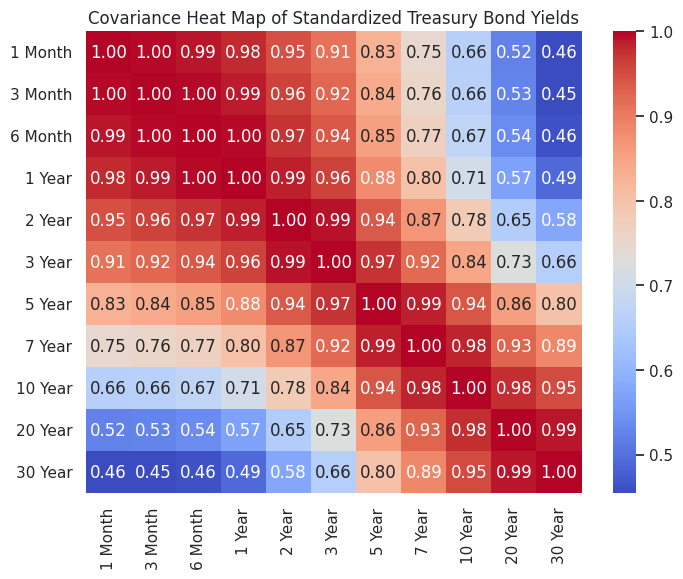
\includegraphics[width=1\textwidth]{gfx/m1l4_notes_covariance_heatmap_standardized.png}
    \caption{Bản đồ nhiệt Hiệp phương sai của Lợi suất Trái phiếu Kho bạc đã Chuẩn hóa}
    \label{fig:m1l4_notes_covariance_heatmap_standardized}
\end{figure}

Bây giờ chúng ta hãy tính toán các vector riêng và trị riêng của ma trận hiệp phương sai của tập dữ liệu lợi suất đã được chuẩn hóa.

\begin{lstlisting}[language=Python]
In [15]: # Calculate eigenvectors and eigenvalues of the covariance matrix of standar
         eigenvalues, eigenvectors = LA.eig(std_data_cov)
         eigenvalues
\end{lstlisting}

\begin{lstlisting}[language=Python]
Out [15]: array([9.22236235e+00, 1.63341019e+00, 1.17347718e-01, 1.46747161e-02,
                 5.37172584e-03, 3.70149555e-03, 1.61309240e-03, 6.97458739e-04,
                 4.12103724e-04, 2.47130907e-04, 1.62022336e-04])
\end{lstlisting}

\begin{lstlisting}[language=Python]
In [16]: eigenvectors
\end{lstlisting}

\begin{lstlisting}[language=Python]
Out [16]: array([[ 0.44114252,  0.16709103, -0.53274513,  0.29838306,  0.30407626,
                  -0.06687106,  0.02716335,  0.33473909, -0.24039038,  0.3702677 ,
                  -0.00401581],
                 [ 0.30709453,  0.3256805 ,  0.3004742 , -0.10407045, -0.09017425,
                  -0.45363295,  0.58333199, -0.13905681, -0.13428768,  0.31674937,
                   0.08135824],
                 [ 0.30335843,  0.29873569,  0.17614053,  0.25730089, -0.24045099,
                  -0.34295333, -0.10807462, -0.13460411,  0.32846299, -0.58367918,
                  -0.26019232],
                 [ 0.42112655, -0.09742097, -0.00945148,  0.26727645,  0.30894871,
                  -0.16475673,  0.38500876,  0.15471834, -0.48093818, -0.17006916,
                   0.43202651],
                 [ 0.31879358,  0.17616334, -0.28944958,  0.31333639,  0.25331718,
                   0.2316792 ,  0.23709616,  0.21742618, -0.3594238 ,  0.02750551,
                  -0.57801452],
                 [ 0.32383758,  0.08574516, -0.41253571,  0.06981027,  0.2557664 ,
                   0.27857918, -0.04283274,  0.253605  ,  0.24613993, -0.32221553,
                   0.58235483],
                 [ 0.32393331, -0.09082567, -0.38335179, -0.28984745,  0.02440707,
                   0.41667104, -0.0335848 , -0.25924506, -0.22190129,  0.51816781,
                  -0.30913315],
                 [ 0.31475338, -0.2155924 , -0.25536488, -0.38788729, -0.13245802,
                  -0.19980121, -0.25664372, -0.23752598, -0.60974821, -0.28958861,
                   0.05811859],
                 [ 0.27752025,  0.29830301, -0.32947806, -0.0224116 , -0.14078023,
                   0.07495589, -0.36651204,  0.64790245,  0.35934669,  0.10798909,
                   0.06783763],
                 [-0.48820444,  0.2677569 , -0.44896794,  0.22584655,  0.25821905,
                   0.02106533,  0.58883593, -0.14816743, -0.03038806,  0.00408296,
                  -0.02532805],
                 [ 0.24905042, -0.49930724,  0.38802724,  0.65844796,  0.19437911,
                  -0.01338036,  0.03078012, -0.21614344, -0.11702391, -0.07221199,
                   0.00323551]])
\end{lstlisting}

Từ output trên, chúng ta có thể thấy các trị riêng và các vector riêng tương ứng của nó đã được sắp xếp theo thứ tự giảm dần dựa trên giá trị của trị riêng. Trong thuật toán PCA, chúng ta cũng gọi các vector riêng là tải số (loadings). Chúng ta sẽ hiểu lý do tại sao điều này lại quan trọng ở phần sau.

Chúng ta có thể coi bộ sưu tập tất cả các vector riêng này như một ma trận biến đổi tuyến tính đối với tập dữ liệu đã chuẩn hóa. Dữ liệu đã được biến đổi này sẽ có một đặc tính rất thú vị mà chúng ta sẽ sớm giới thiệu. Đầu tiên, hãy biến đổi dữ liệu đã chuẩn hóa bằng các vector riêng.

\begin{lstlisting}[language=Python]
In [17]: # Transform standardized data with Loadings
         principal_components = standardized_data.dot(eigenvectors)
         principal_components.columns = ["PC_1", "PC_2", "PC_3", "PC_4", "PC_5", "PC_6",
         principal_components.head()
\end{lstlisting}

\begin{lstlisting}[language=Python]
Out [17]:             PC_1      PC_2      PC_3      PC_4      PC_5      PC_6      PC_7
          2001-07-31  4.608202 -0.918184  0.138746 -0.223360  0.013690  0.063247  0.008572
          2001-08-01  4.665170 -0.950595  0.102492 -0.220182  0.013318  0.054096  0.014505
          2001-08-02  4.766161 -1.009754  0.054519 -0.230244  0.021179  0.064157  0.017119
          2001-08-03  4.807092 -1.038602  0.027695 -0.224234  0.025575  0.063723  0.018644
          2001-08-06  4.781112 -1.044855  0.048161 -0.228694  0.013594  0.051783  0.009102
\end{lstlisting}

Kết quả trên hiển thị 11 biến đã được biến đổi. Trong PCA, chúng được gọi là các thành phần chính (principal components). Hãy nhớ rằng chúng ta đã đề cập trước đó rằng các trị riêng từ PCA được sắp xếp theo thứ tự giảm dần. Những thành phần chính này cũng được trình bày theo cùng trình tự như các trị riêng tương ứng của chúng. Ví dụ, PC\_1 tương ứng với trị riêng đầu tiên, có giá trị là 9.22. PC\_2 tương ứng với trị riêng cao thứ hai, có giá trị là 1.63.

Đặc trưng quan trọng nhất của PCA là các thành phần chính đứng đầu có khả năng giải thích một tỷ lệ phương sai của tập dữ liệu cao hơn so với các thành phần chính còn lại. Ví dụ, PC\_1 có thể giải thích được nhiều sự biến thiên trong dữ liệu đã chuẩn hóa hơn so với PC\_2. Nhưng là bao nhiêu? Trị riêng tương ứng cho PC\_1 chính là lượng phương sai của toàn bộ dữ liệu mà PC\_1 giải thích được. Nó có giá trị 9.22 trong trường hợp này. Theo cùng một logic, PC\_2 giải thích 1.63 trong tổng phương sai của tập dữ liệu. Chúng ta có thể cộng tất cả các trị riêng lại để có được tổng phương sai của dữ liệu. Từ tổng phương sai của dữ liệu, chúng ta cũng có thể tính được tỷ lệ phần trăm đóng góp vào phương sai mà mỗi thành phần chính nắm bắt được. Dưới đây là mã Python.

\begin{lstlisting}[language=Python]
In [18]: # Put data into a DataFrame
         df_eigval = pd.DataFrame({"Eigenvalues": eigenvalues}, index=range(1,12))
         # Work out explained proportion
         df_eigval["Explained proportion"] = df_eigval["Eigenvalues"] / np.sum(eigenv
         #Format as percentage
         df_eigval.style.format({"Explained proportion": "{:.2%}"})
\end{lstlisting}

\begin{lstlisting}[language=Python]
Out [18]:      Eigenvalues  Explained proportion
          1     9.222362      83.84%
          2     1.633410      14.85%
          3     0.117348       1.07%
          4     0.014675       0.13%
          5     0.005372       0.05%
          6     0.003701       0.03%
          7     0.001613       0.01%
          8     0.000697       0.01%
          9     0.000412       0.00%
          10    0.000247       0.00%
          11    0.000162       0.00%
\end{lstlisting}

Từ bảng trên, chúng ta có thể thấy PC\_1 có thể giải thích gần 84\% phương sai trong tập dữ liệu đã chuẩn hóa. PC\_2 có thể giải thích gần 15\% phương sai trong dữ liệu đã chuẩn hóa. Hai thành phần chính đầu tiên này có thể giải thích tới gần 99\% sự biến thiên trong tập dữ liệu. 9 thành phần chính còn lại chỉ giải thích vỏn vẹn 1\% phương sai của dữ liệu. Vì vậy, để phân tích dữ liệu hiệu quả hơn mà không làm mất đi quá nhiều thông tin, chúng ta có thể chỉ sử dụng hai thành phần chính đầu tiên cho việc phân tích thay vì dùng tất cả 11 thành phần chính. Bởi tính chất đặc biệt này, chúng ta cũng gọi PCA là một kỹ thuật giảm chiều dữ liệu.

Phạm vi ứng dụng của PCA rất rộng trong phân tích tài chính và học máy (machine learning). Ví dụ, trong phân tích hình ảnh, bộ sưu tập hình ảnh gốc có thể rất lớn, nhưng bằng cách sử dụng PCA, chúng ta có thể giảm kích thước dữ liệu mà vẫn giữ nguyên được những đặc trưng chính của các hình ảnh.

\subsection{Phân tích Thành phần Chính cho Lợi suất Trái phiếu Kho bạc Hoa Kỳ}

Điều tuyệt vời của việc sử dụng PCA để phân tích đường cong lợi suất Trái phiếu Kho bạc Hoa Kỳ là nó có thể phân tách đường cong lợi suất thành một số các thành phần chính (Oprea). Ba thành phần chính dẫn đầu mô tả các đặc điểm sau đây của đường cong lợi suất:
1. PC\_1: sự dịch chuyển song song của đường cong lợi suất (shift).
2. PC\_2: sự dẹt đi (flattening) hoặc dốc hơn (steeping) của đường cong lợi suất (tilt).
3. PC\_3: sự thay đổi độ cong của đường cong lợi suất (twist).

Đầu tiên, hãy vẽ đường cong lợi suất làm tiêu chuẩn để so sánh tốt hơn (Bjerring).

\begin{lstlisting}[language=Python]
In [19]: # Treasury Yield Curve
         yields.plot(figsize=(12, 8), title='Figure 2, Treasury Yields', alpha=0.7) #
         plt.legend(bbox_to_anchor=(1.03,1))
         plt.show()
\end{lstlisting}

\begin{figure}[htbp]
    \centering
    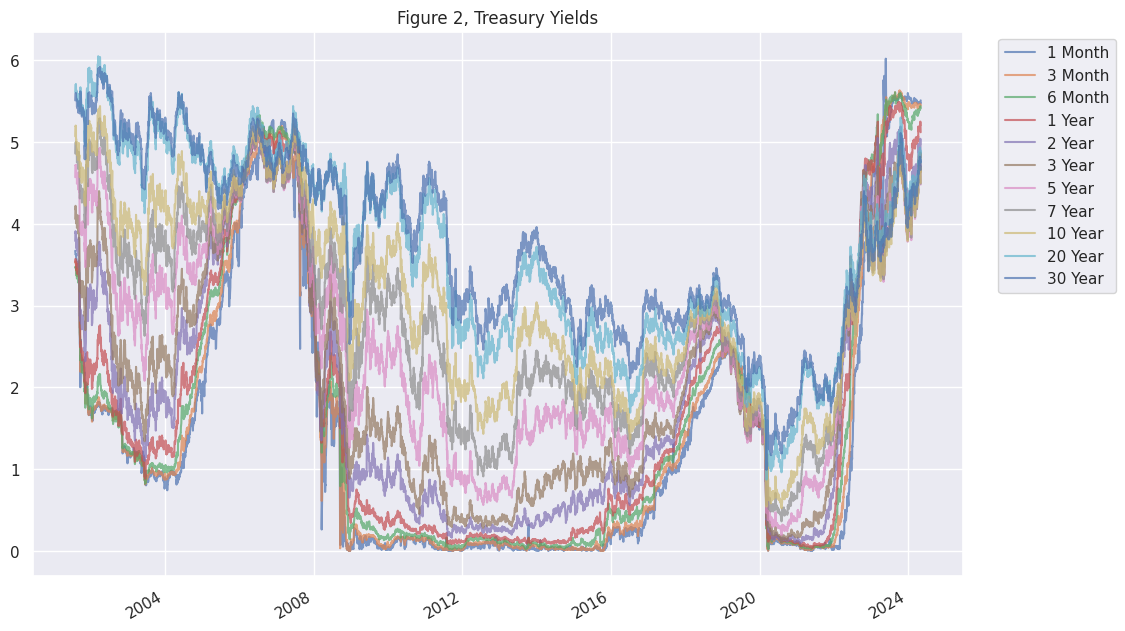
\includegraphics[width=1\textwidth]{gfx/m1l4_notes_fig2_treasury_yields.png}
    \caption{Hình 2, Lợi suất Trái phiếu Kho bạc}
    \label{fig:m1l4_notes_fig2_treasury_yields}
\end{figure}

Bây giờ, hãy vẽ các thành phần chính. Bắt đầu với PC\_1.

\begin{lstlisting}[language=Python]
In [20]: # Plot PC_1
         principal_components["PC_1"].plot(figsize=(12,8), title='Figure 3, Principa
         plt.show()
\end{lstlisting}

\begin{figure}[htbp]
    \centering
    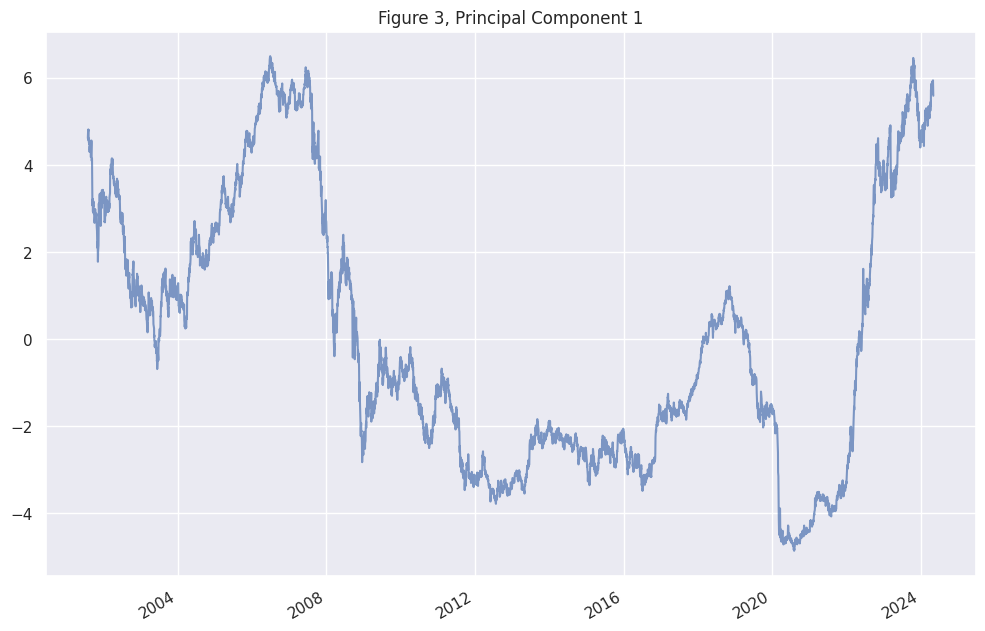
\includegraphics[width=1\textwidth]{gfx/m1l4_notes_fig3_pc1.png}
    \caption{Hình 3, Thành phần Chính 1}
    \label{fig:m1l4_notes_fig3_pc1}
\end{figure}

Từ Hình 3 của PC\_1 ở trên, chúng ta có thể thấy mô hình (pattern) trông tương tự với mô hình của Hình 2 (biểu đồ này bắt đầu từ năm 2001 vì chúng ta đã loại bỏ dữ liệu NaN). PC\_1 này được dùng để thể hiện sự dịch chuyển song song của đường cong lợi suất. Tiếp theo, hãy phân tích PC\_2. PC\_2 thường được dùng để phân tích xem đường cong lợi suất bị nghiêng (tilted) như thế nào. Minh họa bằng mã Python sau đây sẽ giải thích lý do tại sao PC\_2 lại được dùng để phân tích độ nghiêng (tilt).

Đầu tiên, hãy tính toán sự chênh lệch giữa lợi suất 2 năm và lợi suất 10 năm như là độ nghiêng của đường cong lợi suất và vẽ một đồ thị.

\begin{lstlisting}[language=Python]
In [21]: # Calculate slope (difference) of 2-year Treasury yield and 10-year Treasury
         df_s = pd.DataFrame(data = standardized_data)
         df_s = df_s[["2 Year", "10 Year"]]
         df_s["Tilt"] = df_s["2 Year"] - df_s["10 Year"]
         df_s.head()
\end{lstlisting}

\begin{lstlisting}[language=Python]
Out [21]:              2 Year   10 Year      Tilt
          2001-07-31 1.219431  1.687817 -0.468386
          2001-08-01 1.245314  1.721886 -0.476571
          2001-08-02 1.284139  1.772989 -0.488850
          2001-08-03 1.297080  1.798541 -0.501460
          2001-08-06 1.277668  1.790023 -0.512355
\end{lstlisting}

\begin{lstlisting}[language=Python]
In [22]: # Draw the graph of Slope of 2-Year Treasury Yield - 10-Year Treasury Yield
         df_s["Tilt"].plot(figsize=(12,8), title='Figure 4, Tilt of 2-Year Treasury 
         plt.show()
\end{lstlisting}

\begin{figure}[htbp]
    \centering
    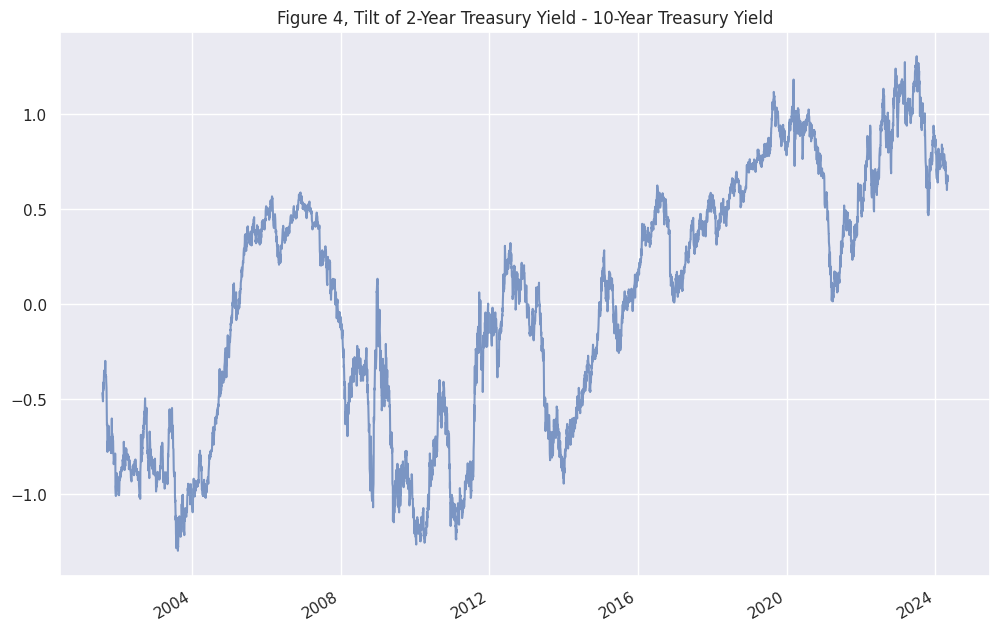
\includegraphics[width=1\textwidth]{gfx/m1l4_notes_fig4_tilt_2y10y.png}
    \caption{Hình 4, Độ nghiêng của Lợi suất Trái phiếu Kho bạc 2 Năm - Lợi suất Trái phiếu Kho bạc 10 Năm}
    \label{fig:m1l4_notes_fig4_tilt_2y10y}
\end{figure}

Sau khi vẽ Hình 4 về mức chênh lệch lợi suất giữa lợi suất Trái phiếu Kho bạc 2 năm và lợi suất Trái phiếu Kho bạc 10 năm, chúng ta hãy vẽ đồ thị cho PC\_2.

\begin{lstlisting}[language=Python]
In [23]: # Draw the graph for PC_2
         principal_components["PC_2"].plot(figsize=(12,8), title='Figure 5, Principa
         plt.show()
\end{lstlisting}

\begin{figure}[htbp]
    \centering
    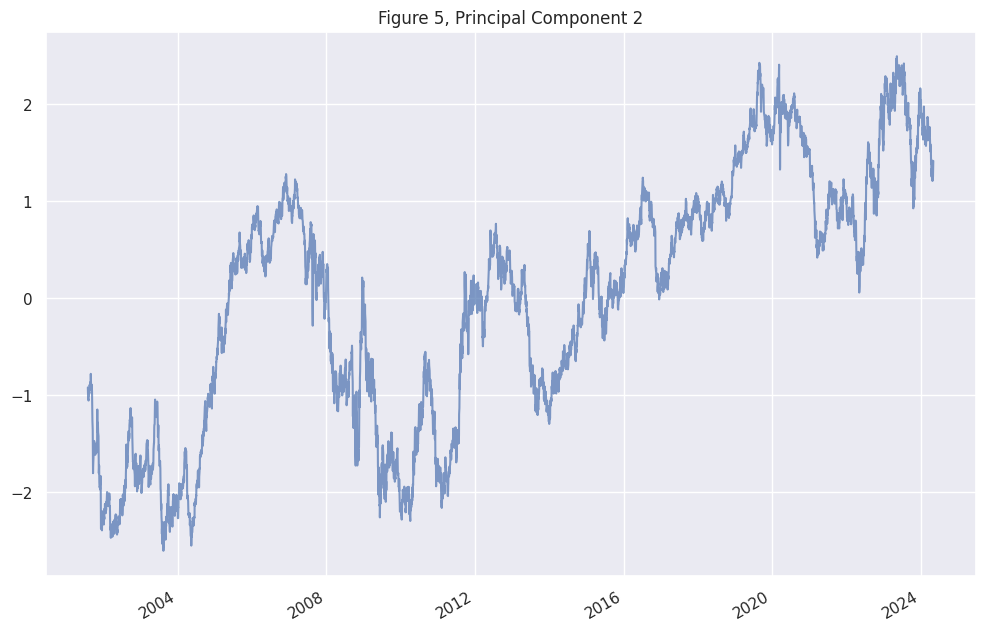
\includegraphics[width=1\textwidth]{gfx/m1l4_notes_fig5_pc2.png}
    \caption{Hình 5, Thành phần Chính 2}
    \label{fig:m1l4_notes_fig5_pc2}
\end{figure}

Từ Hình 4 và Hình 5, chúng ta có thể thấy biểu đồ độ nghiêng (tilt) của lợi suất Trái phiếu Kho bạc 2 năm và lợi suất 10 năm có mô hình tương tự như biểu đồ PC\_2. Hãy tính tương quan để xác nhận quan sát này.

\begin{lstlisting}[language=Python]
In [24]: np.corrcoef(principal_components["PC_2"], df_s["Tilt"])
\end{lstlisting}

\begin{lstlisting}[language=Python]
Out [24]: array([[1.        , 0.97850538],
                 [0.97850538, 1.        ]])
\end{lstlisting}

Đoạn code trên cho thấy rằng tương quan giữa PC\_2 và Độ nghiêng (Tilt) là 97\%, đây là mức rất cao. Vì vậy, chúng ta có thể sử dụng PC\_2 làm đại diện (proxy) để phân tích xem đường cong lợi suất đang nghiêng (tilted) như thế nào.

Bây giờ chúng ta hãy vẽ PC\_3, sự thay đổi độ cong của đường cong lợi suất.

\begin{lstlisting}[language=Python]
In [25]: # Draw the graph for PC_3
         principal_components["PC_3"].plot(figsize=(12,8), title='Figure 6, Principa
         plt.show()
\end{lstlisting}

\begin{figure}[htbp]
    \centering
    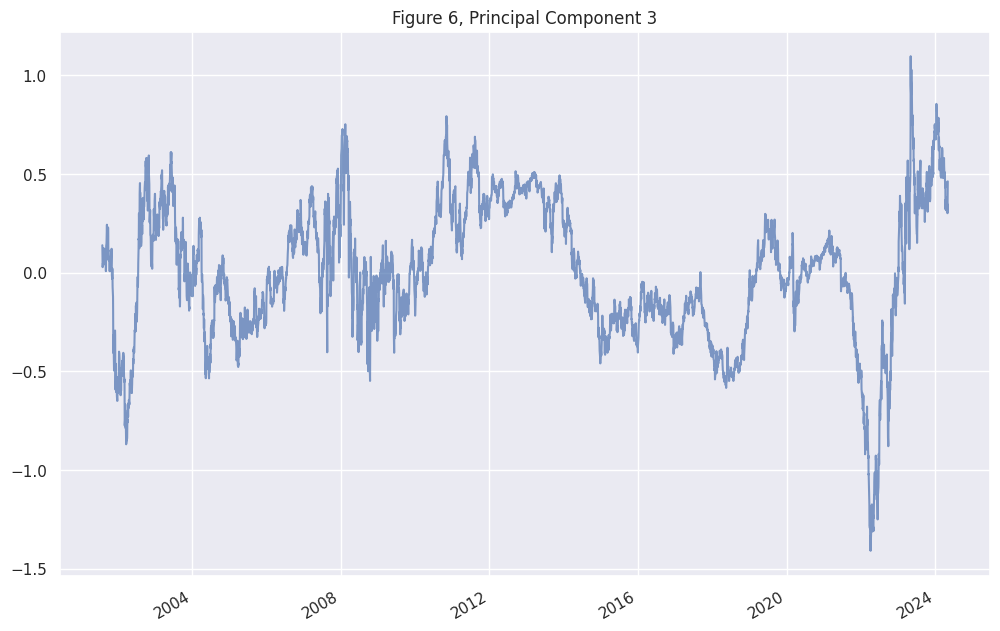
\includegraphics[width=1\textwidth]{gfx/m1l4_notes_fig6_pc3.png}
    \caption{Hình 6, Thành phần Chính 3}
    \label{fig:m1l4_notes_fig6_pc3}
\end{figure}

Từ Hình 6, chúng ta có thể thấy rằng sự thay đổi độ cong của đường cong lợi suất dao động quanh mức 0.

\section[Giá trị Rủi ro cho một Danh mục Đầu tư Có Thu nhập Cố định]{Giá trị Rủi ro (Value at Risk) cho một Danh mục Đầu tư Có Thu nhập Cố định}

Trong phần này, chúng ta sẽ sử dụng phương pháp trích xuất đặc trưng mà chúng ta đã học ở phần trước để tính toán Giá trị Rủi ro (Value at Risk) của một danh mục đầu tư trái phiếu.

\subsection[Giá trị Rủi ro]{Giá trị Rủi ro (Value at Risk - VaR)}

Giá trị Rủi ro (VaR) là một thước đo thống kê để đánh giá mức độ tổn thất tối đa tiềm tàng của một khoản đầu tư hay một danh mục đầu tư trong một khoảng thời gian xác định dưới một mức độ tin cậy (confidence level) nhất định. Ví dụ, khi một danh mục đầu tư cổ phiếu có VaR là 1 triệu đô la trong một ngày ở mức độ tin cậy 95\%, điều đó có nghĩa là có 95\% xác suất danh mục đầu tư cổ phiếu này sẽ không mất hơn 1 triệu đô la trong một ngày.

VaR là một chỉ số rủi ro dễ hiểu và có thể được sử dụng để so sánh rủi ro trên các nhóm tài sản khác nhau. VaR thường được sử dụng trong quản trị rủi ro đối với quản lý danh mục đầu tư hoặc cho các báo cáo quy định. Nó cũng là một phần của các thước đo nhằm thiết lập mức trần rủi ro (risk cap) cho các nhà giao dịch. VaR cũng có thể được áp dụng cho việc phân bổ vốn.

\subsection{VaR đối với một Danh mục Đầu tư Trái phiếu Kho bạc Đơn giản}

Chúng ta sẽ chỉ ra cách tính VaR cho một danh mục đầu tư Trái phiếu Kho bạc đơn giản trong phần này. Danh mục đầu tư trái phiếu đơn giản này sẽ chỉ bao gồm Trái phiếu Kho bạc kỳ hạn 2 năm, Trái phiếu Kho bạc kỳ hạn 5 năm, và Trái phiếu Kho bạc kỳ hạn 10 năm. Đầu tiên, hãy tạo một tập dữ liệu với lợi suất của ba trái phiếu này và tính tỷ lệ phần trăm thay đổi lợi suất hàng ngày của chúng.

\begin{lstlisting}[language=Python]
In [26]: # Create a dataset with 3 Treasury bond yields and calculate the yield chang
         var_dataset = yields[["2 Year", "5 Year", "10 Year"]]
         var_yield_chng_dataset = var_dataset.pct_change()
         var_yield_chng_dataset = var_yield_chng_dataset.dropna()
         var_yield_chng_dataset.head()
\end{lstlisting}

\begin{lstlisting}[language=Python]
Out [26]:               2 Year    5 Year   10 Year
          2001-08-01  0.010554  0.010941  0.007890
          2001-08-02  0.015666  0.015152  0.011742
          2001-08-03  0.005141  0.006397  0.005803
          2001-08-06 -0.007673 -0.002119 -0.001923
          2001-08-07  0.005155  0.002123  0.001927
\end{lstlisting}

Tiếp theo, chúng ta sẽ chuẩn bị tập dữ liệu. Đầu tiên chúng ta cần chuẩn hóa dữ liệu.

\begin{lstlisting}[language=Python]
In [27]: # Standardize the dataset
         var_yield_chng_dataset_means = var_yield_chng_dataset.mean()
         var_yield_chng_dataset_stds = var_yield_chng_dataset.std()
         var_yld_chng_stnd_data = (var_yield_chng_dataset - var_yield_chng_dataset_me
\end{lstlisting}

Bây giờ chúng ta có thể tính toán các vector riêng và trị riêng của tập dữ liệu đã được chuẩn hóa.

\begin{lstlisting}[language=Python]
In [28]: # Calculate eienvectors and eigenvalues and rank by eigenvalues
         var_cov_matrix = var_yld_chng_stnd_data.cov()
         eigenvalues, eigenvectors = np.linalg.eig(var_cov_matrix)
         sorted_indices = np.argsort(eigenvalues)[::-1]
         pca_components = eigenvectors[:, sorted_indices]
\end{lstlisting}

Hãy cùng kiểm tra các trị riêng và xem mỗi vector riêng có khả năng giải thích bao nhiêu phần trăm phương sai của dữ liệu.

\begin{lstlisting}[language=Python]
In [29]: # Put data into a DataFrame
         df_eigval = pd.DataFrame({"Eigenvalues": eigenvalues}, index=range(1,4))
         # Work out explained proportion
         df_eigval["Explained proportion"] = df_eigval["Eigenvalues"] / np.sum(eigenv
         #Format as percentage
         df_eigval.style.format({"Explained proportion": "{:.2%}"})
\end{lstlisting}

\begin{lstlisting}[language=Python]
Out [29]:      Eigenvalues  Explained proportion
          1     2.545146      84.84%
          2     0.384763      12.83%
          3     0.070091       2.34%
\end{lstlisting}

Từ bảng trên, chúng ta có thể thấy hai vector riêng đầu tiên chiếm tới 97\% phương sai trong tập dữ liệu. Vì vậy, chúng ta sẽ chọn hai vector riêng đầu tiên này để phân tích.

\begin{lstlisting}[language=Python]
In [30]: # Choose number of components (e.g., 2)
         n_components = 2
         selected_components = pca_components[:, :n_components]
\end{lstlisting}

Tiếp theo, hãy giả sử rằng danh mục đầu tư trái phiếu đơn giản của chúng ta bao gồm 2 triệu đô la Trái phiếu Kho bạc kỳ hạn 2 năm, 2 triệu đô la Trái phiếu Kho bạc kỳ hạn 5 năm, và 1 triệu đô la Trái phiếu Kho bạc kỳ hạn 10 năm.

\begin{lstlisting}[language=Python]
In [31]: # Define a simple portfolio
         portfolio = {
             2: 2000000,   # $2M in 2-year bond
             5: 2000000,   # $2M in 5-year bond
             10: 1000000   # $1M in 10-year bond
         }
\end{lstlisting}

Tiếp đến, chúng ta sẽ tính các độ nhạy cảm của trái phiếu (bond sensitivities) trong danh mục đầu tư. Để đơn giản hóa, chúng ta giả định khoảng thời gian đáo hạn bình quân (duration) của trái phiếu bằng đúng kỳ hạn của chúng. Khi đó, chúng ta có thể tính được những thay đổi về giá trị của danh mục đầu tư và VaR.

\begin{lstlisting}[language=Python]
In [32]: # Calculate portfolio sensitivities (assuming duration = maturity for simpli
         sensitivities = np.array([maturity * amount for maturity, amount in portfoli
         
         # Calculate portfolio value changes
         portfolio_changes = (var_yield_chng_dataset * sensitivities) @ selected_compor
         
         # Calculate VaR
         confidence_level = 0.95 # 95% VaR
         var = -np.percentile(portfolio_changes, 100 * (1 - confidence_level))
         print(f"1-day 95% VaR: ${var:,.2f}")
         
         # Display summary statistics
         print("\nSummary Statistics:")
         print(f"Portfolio Value: ${sum(portfolio.values()):,.2f}")
         print(f"VaR as % of Portfolio Value: {var / sum(portfolio.values()) * 100:.3f}%")
\end{lstlisting}

\begin{lstlisting}[language=Python]
1-day 95% VaR: $458,248.59

Summary Statistics:
Portfolio Value: $5,000,000.00
VaR as % of Portfolio Value: 9.165%
\end{lstlisting}

Kết quả trên cho thấy VaR 1 ngày ở mức độ tin cậy 95\% cho danh mục đầu tư Trái phiếu Kho bạc đơn giản của chúng ta là \$458.249. Con số này tương đương khoảng 9\% tổng giá trị danh mục đầu tư. Ví dụ trên minh họa cách sử dụng phương pháp trích xuất đặc trưng để thu gọn tập dữ liệu danh mục đầu tư và sử dụng tập dữ liệu nhỏ hơn đó để tính toán VaR.

\section[Kết luận]{Kết luận (Conclusion)}

Trong bài học này, trước tiên chúng ta đã đi qua những kiến thức cơ bản về phân tích biến đôi. Chúng ta đã giải thích phân tích biến đôi là gì và sau đó giới thiệu các khái niệm hiệp phương sai và tương quan. Tiếp theo, chúng ta chuyển sang việc áp dụng phương pháp trích xuất đặc trưng để phân tích đường cong lợi suất Trái phiếu Kho bạc. Chúng ta đã học cách chuẩn hóa một tập dữ liệu. Chúng ta cũng đã học về vector riêng và trị riêng. Sau đó, chúng ta đã tiến hành trích xuất đặc trưng từ lợi suất trái phiếu Kho bạc. Kế tiếp, chúng ta cũng áp dụng phương pháp trích xuất đặc trưng để tính toán Giá trị Rủi ro (Value at Risk) của một danh mục đầu tư trái phiếu Kho bạc đơn giản. Những công cụ này là nền tảng cốt lõi để hiểu được các lý thuyết tài chính ở cấp độ nâng cao hơn.

\section*{Tài liệu tham khảo (References)}

\begin{itemize}
    \item Bjerring, Thomas T. "The Yield Curve and Its Components." Github, 16 October 2019, \url{https://bjerring.github.io/bonds/2019/10/16/the-yield-curve-and-its-components.html}.
    \item Oprea, Andreea. "The Use of Principal Component Analysis (PCA) in Building Yield Curve Scenarios and Identifying Relative-Value Trading Opportunities on the Romanian Government Bond Market." Journal of Risk and Financial Management, vol. 15, no. 6, 2022. \url{https://www.mdpi.com/1911-8074/15/6/247}.
\end{itemize}

Copyright 2024 WorldQuant University. This content is licensed solely for personal use. Redistribution or publication of this material is strictly prohibited.
